
\section{Background}

The Internet of Things (IoT) industry has grown exponentially over the last few years resulting in a more seamlessly integrated digital world. One major development stunt in the IoT industry has been caused by the inability to integrate micropayment methods between devices in a reliable, secure and cost-effective way. A possible solution to this problem could be developed through the use of new technologies such as blockchain and payment channel technologies. With these tools, IoT devices could easily make micropayments between each other which would allow for a range of applications such as pay-as-you-go services for the use of data, sensors, electricity and more.

\section{Problem statement}

The Bitcoin blockchain and Lightning Network are very new technologies and so very little has been done in term of using these technologies  to facilitate micropayments for IoT devices. The aim of this report is thus to explore the possible integration of these technologies with IoT devices to facilitate micropayments and then to evaluate whether or not the payment solution that these technologies offer is better or worse than the current payment methods being used.

\section{Problem objectives}

The objective of this project is first to understand the details of Bitcoin and the Lightning network and then to implement a simple IoT system that will use these technologies to facilitate micropayments. A user of this system should be able to use and be charged for a resource on a pay-as-you consume basis.

\section{Scope and limitations}

The Lightning Network is a very new technology and so is still in the process of development and can not yet be completely trusted to be secure. Thus for the sake of this project, only the Bitcoin testnet and Lightning testnet will be used and so only value-less testnet Bitcoins will be used during  the testing of the implementation.

The Lightning	Network implementations that exist still are known to have occasional issues with routing payment channels. These problems lie outside the scope of this investigation.


\section{Plan of development}

[TO DO]

\begin{figure}[h]
\centering
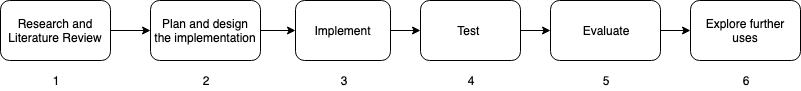
\includegraphics[scale=0.5]{Figures/plan_of_development.jpg}
\caption{Diagram showing the plan of development}
\label{fig:plan_of_development}
\end{figure}
